\documentclass[11pt]{amsart}
\usepackage{geometry}                % See geometry.pdf to learn the layout options. There are lots.
\geometry{letterpaper}                   % ... or a4paper or a5paper or ... 
%\geometry{landscape}                % Activate for for rotated page geometry
%\usepackage[parfill]{parskip}    % Activate to begin paragraphs with an empty line rather than an indent
\usepackage{graphicx}
\usepackage{tikz}
\usepackage{amssymb}
\usepackage{bbold}
\usepackage{epstopdf}
\DeclareGraphicsRule{.tif}{png}{.png}{`convert #1 `dirname #1`/`basename #1 .tif`.png}

\title{Memoir on Information of CRN}
\author{Filipe}
%\date{}                                           % Activate to display a given date or no date

\begin{document}
\maketitle
\section{Case of study (Michaelis-Menten mechanism)}
The mechanism is
\begin{equation}
E + S \underset{k_{-1}}{\overset{k_{+1}}{\rightleftharpoons}} ES  \underset{k_{-2}}{\overset{k_{+2}}{\rightleftharpoons}} E + P
\end{equation}

\begin{itemize}
\item We assume $S$ and $P$ to be chemostated (fixed concentration/copy numbers).
\item There's a single molecule of each enzyme ($E$) or enzyme complexed ($ES$).
\item The system has 2 states, either in $E$ or $ES$.
\end{itemize}

\subsection{Posing the problem}
\begin{itemize}
\item What is information in the scenario of the enzyme processing?
\item Can this CRN be seen as a information channel?
\end{itemize}

\section{Insights from information theory}
A similar system is the Binary Symmetric Channel (BSC), which we'll try to construct an analogy with.

\begin{figure*}[h]
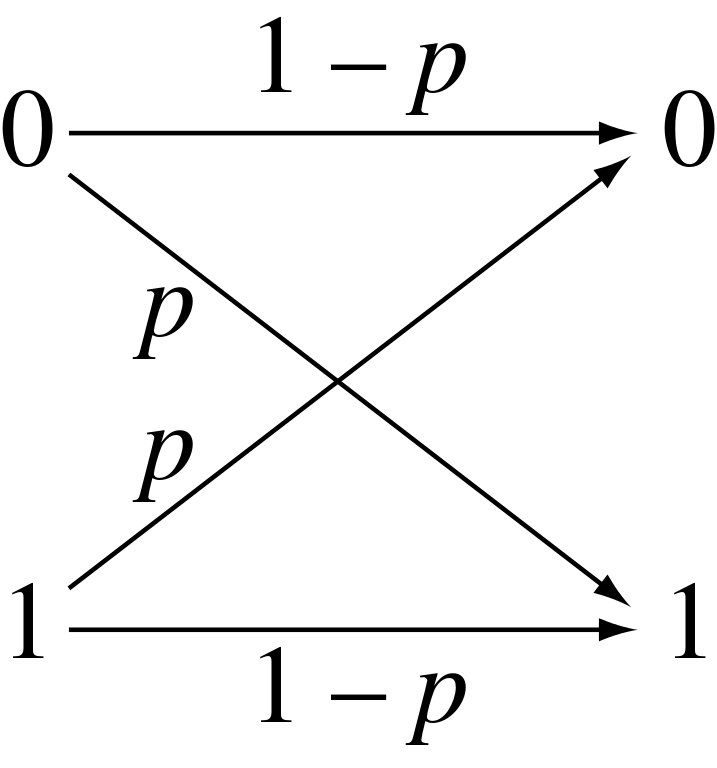
\includegraphics[scale=.1]{Binary_symmetric_channel}
\end{figure*}

\subsection{Binary Symmetric Channel}
Suppose a channe that transmits one single bit per usage (cycle).

\begin{itemize}
\item The probability of sending either 0 or 1 and receiving the same thing is
$$Pr\{Y = 0 | X = 0\} = Pr\{Y = 1 | X = 1\} = 1- p.$$

\item Otherwise we obtain an error in the message sent
$$Pr\{Y = 1 | X = 0\} = Pr\{Y = 0 | X = 1\} = p.$$

\item[(!)] The channel is called symmetric because there's no preference for an error or a message to be sent (equiprobable events).
\end{itemize}

The BSC models the behavior of a channel which transmits the output of a system with two states. Let's define

\begin{itemize}
\item ({\bf System/Source}): It has two states $X = {0,1}$. Assuming the probability of them being equal\footnote{We may also say the system splits the {\it phase space} in two, this might be useful later.}:
$$Pr\{X = x\} = 1/2, x \in X.$$
\begin{itemize}
\item The Shannon entropy of the source is 
$$\mathcal{H}(X) = -\sum_{x \in X} Pr\{X=x\} \log Pr\{X=x\}.$$
If we assume base 2 for the $\log$ we obtain that $\mathcal{H}(X) = 1 \, \text{bit}$. That is, we expect to obtain 1 bit of information by measuring the system.
\item The base 2 was chosen because the phase space of the system has size $|X|=2$.\footnote{{\it What would happen if $|X| \rightarrow\infty$?}}
\end{itemize}

\item ({\bf Channel}): It transmites the information from the source. If the channel has a Markovian property, its current state only depends in the previous state, e.g. the BSC.

\begin{itemize}
\item The Mutual Information quantifies the information expected to be acquired about the system $X$ or the output of the channel $Y$ from the observation of $Y$ or $X$
%
$$\begin{aligned}
\mathcal{I}(X;Y) &= D_{KL}(Pr\{X,Y\}||Pr\{X\}Pr\{Y\}) \\
&= \sum_{x \in X, y \in Y} Pr\{X=x, Y=y\} \log \left( \frac{Pr\{X=x, Y=y\}}{Pr\{X\}Pr\{Y\}} \right)
\end{aligned}
$$
being $Pr\{X=x, Y=y\} = Pr\{Y=y | X=x\} Pr\{X=x\}$.

\item If the channel is the BSC, the mutual information is
$$\mathcal{I}(X;Y) = \log 2 + (1-p) \log (1-p) + p \log p.$$
\end{itemize}

\item For $p=0$ there's no error and the message gets through as well as transmitted.
\item For $p=1$, we assume that it is known the channel always ``flip'' the bit, thus the information at the end of the channel is known, but flipped.
\item $\mathcal{I}(X;Y)$ is minimized for $p=1/2$ and the expected information to be acquired with the measurement is null.
\end{itemize}

\section{What means information in the scenario of the Michaelis-Menten mechanism?}

We know the system can be in the states $X = \{E, ES\}$.
\begin{itemize}
\item The reaction of the system will transform (or not) the species $X$ into something else.
\item We can understand this as the action of the channel over the message. The channel can flip (or not) the bit as the reaction can switch (or not) the enzyme to the complexed enzyme.
\end{itemize}

Translating this into probabilities, we understand that:
\begin{itemize}
\item The system can be in $X = \{E, ES\}$.
\item A reaction occurs, and the states at the end of the reaction are $Y = \{E, ES\}$.
\end{itemize}

\vspace{10pt}
Let's suppose that $\tau$ is what is known as the {\it time for the next reaction}, i.e. the time in which only a single reaction fires.

\begin{itemize}
\item Given the system is initially at $X_0$, when a reaction fires the system goes to a state $X_\tau$.
\item The probability of the system being in a state $\{E, ES\}$ after the reaction is given by $Pr\{X_0 = x | X_\tau = x\}$.
\item The solution of the Chemical Master Equation gives us the transition probability of an arbitrary time $t$ after the initial state
$$\frac{\partial}{\partial t} Pr\{X_0 = x | X_t = x\} = \text{TO-DO} \Rightarrow Pr\{X_0 | X_t \} = Pr\{X_0 | X_0 \} e^{Gt},$$
where $G$ is the {\it generator matrix}.
\end{itemize}

\subsection{Information of the Michaelis-Menten}
Once posed the mathematics, we are in position to question what the calculations give us.
\begin{itemize}
\item We can obtain the mutual information about the states of the enzyme at the beginning and after a time $t$.
\item This will give us the expected information to be gained about the initial state by measuring the system at a time $t$, or {\it vice-versa}. Then
$$\mathcal{I}(X_0;X_t) = \sum_{x \in X_0, y \in X_t} Pr\{X_0=x, X_t=y\} \log \left( \frac{Pr\{X_0\!=\!x, X_t\!=\!y\}}{Pr\{X_0\!=\!x\}Pr\{X_t\!=\!y\}} \right),$$
where $Pr\{X_t\! =\!y , X_0\! = \!x\} = Pr\{X_t\! =\!y | X_0\!=\!x\}Pr\{X_0\!=\!x\}$ and $Pr\{X_t\! =\!y\} = \sum_{x \in X} Pr\{X_t\!=\!y , X_0=x\} $.
\end{itemize}

\subsubsection{Evaluation of the quantities}
Let's define:

\begin{itemize}
\item[-] The transition matrix $\left[P\right]_{ij} = Pr\{X_t\! =\!j | X_0\! = \!i\}$;
\item[-] The probability of the initial state $\left[p_0\right]_i =  Pr\{ X_0\! = \!i\}$;
\item[-] The above gives us the joint probability $Pr\{X_t\! =\!j , X_0\! = \!i\}=\left[\text{diag}(p_0)P\right]_{ij}$.
\item[-] The marginalization over $X_0$ is:
$$ Pr\{X_t = j\} = \left[\mathbb{1}^\top \text{diag}(p_0)P\right]_j = \left[p_0P\right]_j, \quad \mathbb{1} = [1, 1, ..., 1]^\top.$$
\end{itemize}

Recap the probability transition of the continuous-time Markov chain (CTMC). Then:
\begin{itemize}
\item[-] The transition probability matrix for a time $t$ as $\left[P_t\right]_{ij} = Pr\{X_t\! =\!j | X_0\! = \!i\}$;
\item[-] $P_t$ is obtained by the solution of an ODE, being $P_t = e^{Gt}$.
\end{itemize}

TO-DO

\subsubsection{Channel capacity}
It is defined as the probability distribution of $X_0$, say $Pr\{X_0\}$, which maximizes the expected information to be acquired from the observation of $X_t$, which reads
$$C = \underset{Pr\{X_0\}}{\text{max}} \mathcal{I}(X_0;X_t).$$

\begin{itemize}
\item ({\bf BSC}): Which $Pr\{X\}$ maximizes the mutual information for the BSC?
\item[-] Let's assume that $Pr\{X = 0\} = f$ and $Pr\{X = 1\} = 1-f$. If the BSC has an error probability of $p=0.15$, then we can verify that $\mathcal{I}(X;Y)$ is maximized for $f=1/2$, the uniform distribution (see D.J.C. MacKay).

\end{itemize}


In Information Theory, this definition makes sense to help us in finding a coding for the source which mitigate the errors of the channel. Such coding scheme has a probability distribution over its words $Pr\{X\}$. In the case of reaction channels we would have initial distributions which would mitigate the information lost about the initial state when reacting\footnote{Think about the definition of the mutual information in terms of the KL-divergence, maximizing the later is the same as increase the ``difference'' in a KL sense between the joint probability of $(X_0,X_t)$ and the product of their marginals, what would imply that they are independent.}. In the figure below it is plotted how $\mathcal{I}(X_0;X_t)$ varies with $f$ for $Pr\{X_0 = E\} = f$ and $Pr\{X_0 = ES\} = 1-f$. By inspection we note that $C$ is maximized when $f \rightarrow 0$.

\begin{figure*}[h]
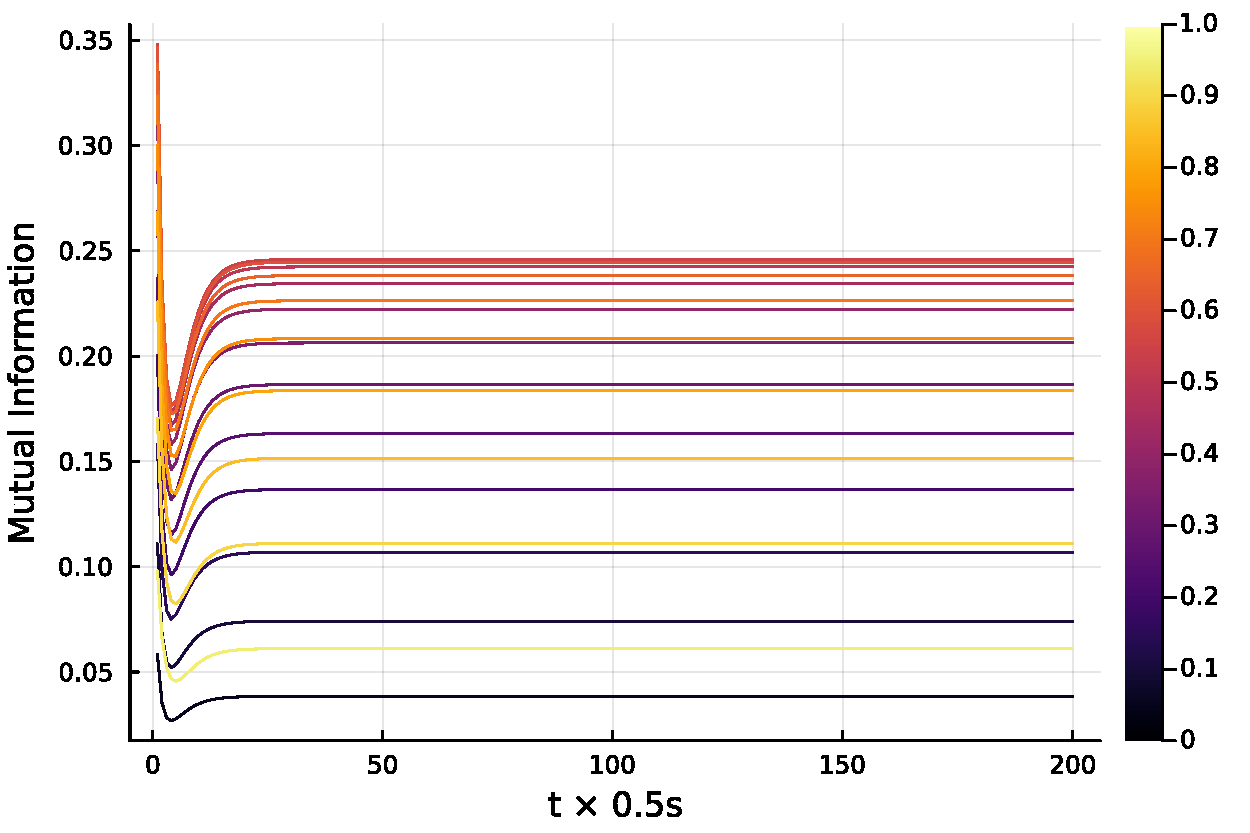
\includegraphics[scale=.5]{I_mutual}
\end{figure*}
\end{document}  